\documentclass[tikz,border=2pt]{standalone}
\usepackage{amsmath}
\usepackage{amssymb}
\usepackage{xcolor}

\definecolor{journalink}{HTML}{1F1C18}
\definecolor{journalmuted}{HTML}{8A7F72}
\definecolor{journalaccent}{HTML}{9C2D2D}

\newcommand{\axisrow}[2]{%
  \draw[journalink, line width=0.8pt, ->, >=stealth] (0,#1) -- (6.4,#1);
  \node[journalink, right] at (6.4,#1) {#2};
  \draw[journalink, line width=0.8pt] (1.0,{#1+0.16}) -- (1.0,{#1-0.16});
  \node[journalink, below, font=\small] at (1.0,{#1-0.16}) {$0$};
  \draw[journalink, line width=0.8pt] (2.4,{#1+0.16}) -- (2.4,{#1-0.16});
  \node[journalink, below, font=\small] at (2.4,{#1-0.16}) {$1$};
  \draw[journalink, line width=0.8pt] (3.8,{#1+0.16}) -- (3.8,{#1-0.16});
  \node[journalink, below, font=\small] at (3.8,{#1-0.16}) {$2$};
  \draw[journalink, line width=0.8pt] (5.2,{#1+0.16}) -- (5.2,{#1-0.16});
  \node[journalink, below, font=\small] at (5.2,{#1-0.16}) {$3$};
}
\newcommand{\segrow}[3]{\draw[journalaccent, line width=1.8pt] (#2,#1) -- (#3,#1);}
\newcommand{\closeddot}[2]{\fill[journalink] (#2,#1) circle (2.2pt);}

\begin{document}
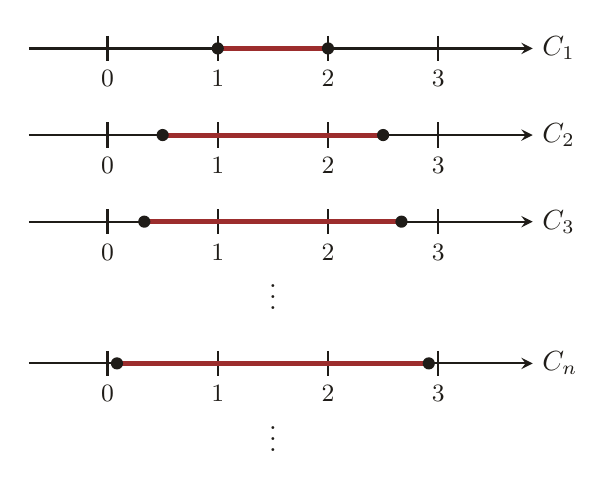
\begin{tikzpicture}[x=1cm, y=1cm, every node/.style={font=\normalsize}]

  \axisrow{0}{$C_1$}
  \segrow{0}{2.4}{3.8}
  \closeddot{0}{2.4}
  \closeddot{0}{3.8}

  \axisrow{-1.1}{$C_2$}
  \segrow{-1.1}{1.7}{4.5}
  \closeddot{-1.1}{1.7}
  \closeddot{-1.1}{4.5}

  \axisrow{-2.2}{$C_3$}
  \segrow{-2.2}{1.467}{4.733}
  \closeddot{-2.2}{1.467}
  \closeddot{-2.2}{4.733}

  \node[journalink] at (3.1,-3.05) {$\vdots$};

  \axisrow{-4.0}{$C_n$}
  \segrow{-4.0}{1.12}{5.08}
  \closeddot{-4.0}{1.12}
  \closeddot{-4.0}{5.08}

  \node[journalink] at (3.1,-4.85) {$\vdots$};

\end{tikzpicture}
\end{document}
